\section{Pianificazione}

Con lo scopo di rispettare le scadenze descritte in questo documento è stata redatta la pianificazione del lavoro traendo ispirazione dalle attività previste nei processi di Fornitura e Sviluppo descritti nello standard ISO/IEC 12207:1995, si organizza la suddivisione del lavoro nelle seguenti macro-fasi:
\begin{itemize}
	\item{\textbf{Attività preliminari di avvio ed analisi dei requisiti;}}
	\item{\textbf{Progettazione architetturale}}
	\item{\textbf{Progettazione di dettaglio e codifica}}
	\item{\textbf{Validazione e collaudo.}}
\end{itemize} 
In base alle scadenze inserite ad inizio documento, le macro-fasi saranno suddivise in questi periodi temporali:
\newline
\begin{table}[h!]
	\centering
	\begin{tabular}{|l|l|l|}
		\hline
		\textbf{Fase} & \textbf{inizio} & \textbf{fine}\\
		\hline
		Attività preliminari di avvio ed analisi dei requisiti & 19/11/2018 & 14/01/2019 \\
		\hline
		Progettazione architetturale & 22/01/2019 & 08/03/2019\\
		\hline
		Progettazione di dettaglio e codifica & 16/03/2019 & 12/04/2019\\
		\hline
		Validazione e collaudo & 20/04/2019 & 10/05/2019\\
		\hline
	\end{tabular}
	\caption{Pianificazione}
\end{table}

Queste fasi vengono inserite in un diagramma di Gantt. Dove le milestone vengono assunte come principali scadenze di ogni fase. Verranno inoltre segnalati con colori diversi quelle scadenze che sono bloccanti oppure no ed  ogni attività è rappresentata tramite le sue sotto attività.
\newline Avendo in mente l'obiettivo di far ricoprire ad ogni membro del gruppo tutti i ruoli, ogni macro-fase è stata divisa in 2 parti, indicativamente della stessa durata, così da avere un momento definito per il cambio i ruoli e per fare una verifica intermedia al periodo per valutare l'avanzamento del lavoro. 

\subsection{Attività preliminari di analisi}
Il periodo preliminare di analisi si svolge dal 19/11/2018 al 14/01/2019 e partono dalla formazione del gruppo terminando poi alla prima milestone ovvero la consegna dei documenti. \newline
In ordine di esecuzione le attività principali sono le seguenti:
\begin{itemize}
	\item{\textbf{Norme di progetto:} questo è il primo documento poiché contiene tutte le norme atte a regolare internamente il gruppo Dream Corp. che spaziano dall'indentatura del codice alle regole per stendere i documenti stessi;}
	\item{\textbf{Studio di fattibilità:} redatta dagli Analisti questa è un' attività bloccante per l'inizio dell'analisi dei requisiti. Consiste in un analisi dei pro ed i contro dei vari capitolati con il fine di una scelta ponderata del capitolato;}
	\item{\textbf{Analisi dei requisiti:} dopo aver scelto il capitolato è necessario approfondire i requisiti richiesti dalla proponente. Svolto ancora una volta dagli Analisti;}
	\item{\textbf{Piano di progetto:} questa attività è bloccante per la stesura della lettera di presentazione. Viene svolta dal Responsabile che ha lo scopo di analizzare le attività necessarie e la loro scadenza al fine di garantire la  buona riuscita del progetto mentre L'amministratore analizza i rischi nei quali il gruppo Dream Corp. può incombere durate il percorso. Inoltre in questa attività vengono stabilite le risorse disponibili per l'intero progetto;}
	\item{\textbf{Piano di qualifica:} in questa attività viene redatto il documento \textit{Piano di Qualifica} che ha lo scopo di individuare dei metodi per garantire la qualità del prodotto;}
	\item{\textbf{Glossario:} questa attività` consiste nella redazione del \textit{Glossario}, dove verranno inseriti tutti i termini considerati possibilmente ambigui;} 
	\item{\textbf{Lettera di presentazione:} attività che consiste nello studio autonomo do ogni membro del gruppo e, sopratutto, nella preparazione del materiale di supporto necessario per la stesura della \textit{Lettera di presentazione} necessaria per il gruppo al fine di essere scelto come fornitore.}
\end{itemize}

\begin{figure}[h!]
	\centering
	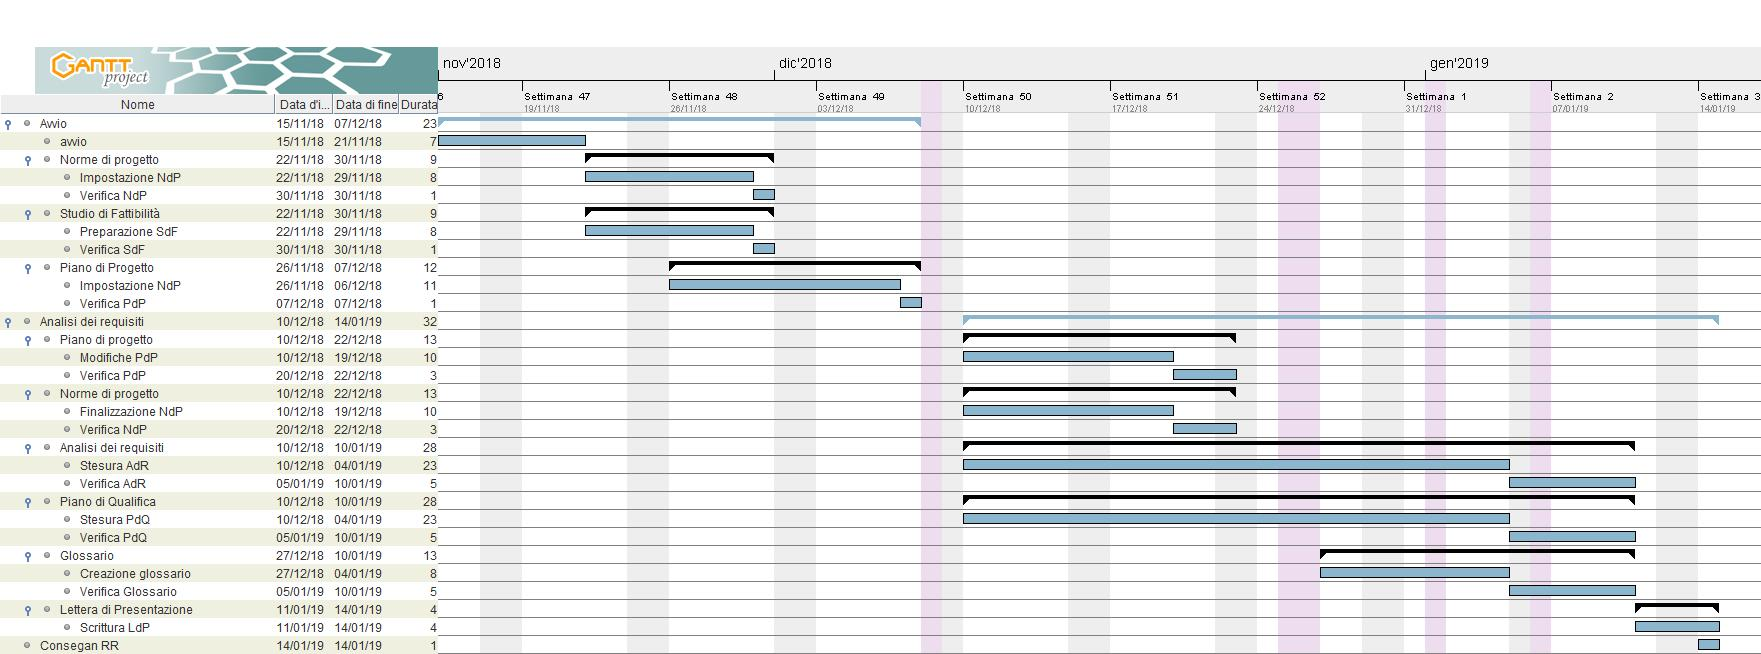
\includegraphics[width=\textwidth]{Gantt_prima_fase.jpg}
	\caption{Diagramma di Gantt per la fase fino alla Revisione dei Requisiti}
\end{figure}

\begin{figure}[h!]
\centering
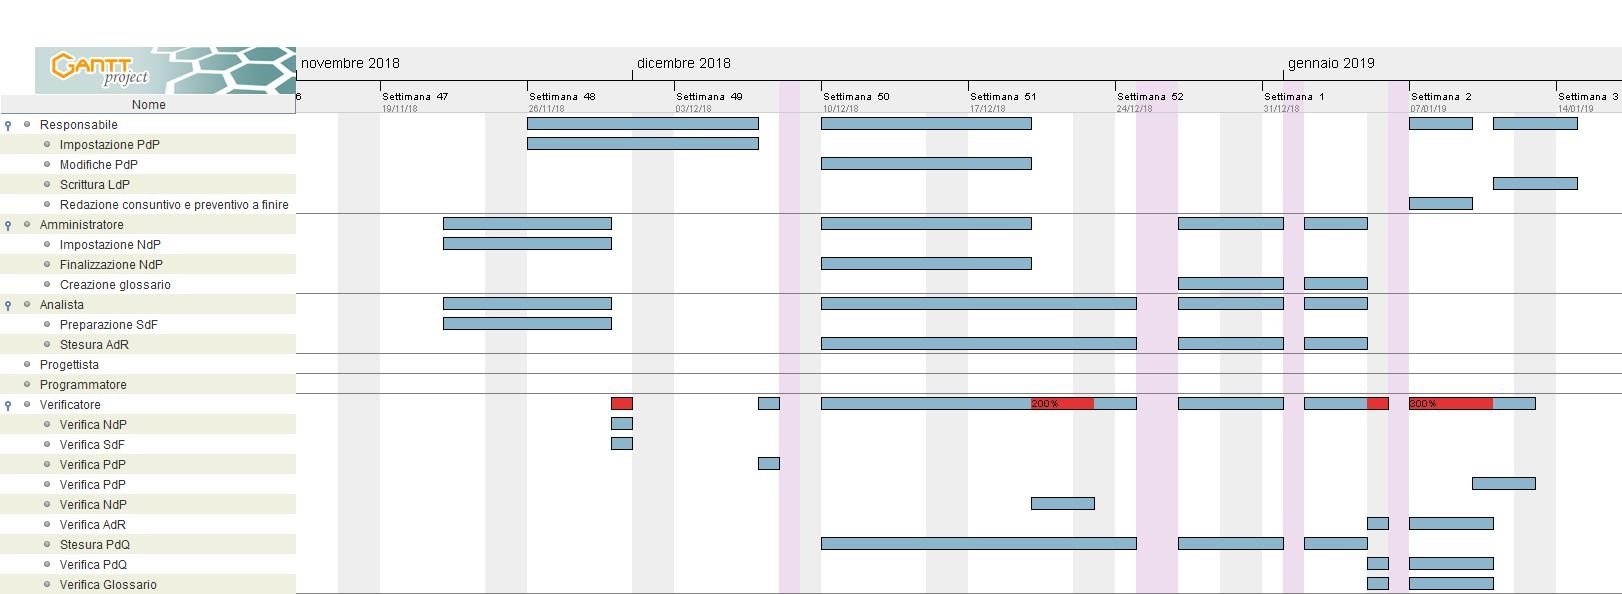
\includegraphics[width=\textwidth]{Gantt_prima_fase_risorse.jpg}
\caption{Diagramma di Gantt delle risorse fino alla Revisione dei Requisiti}
\end{figure}


\begin{table}[h!]
	\centering
	\begin{tabular}{|c|p{4.5cm}|p{4.5cm}|}
		\hline
		\multicolumn{3}{|c|}{\textbf{Suddivisione temporale da rifare}}\\
		\hline
		\textbf{Ruolo} & \textbf{19/11/18 - 20/12/18} & \textbf{20/12/18 - 14/01/19} \\
		\hline
		\textbf{Responsabile} & \pie  & \parbox{4.5cm}{\mic \\\daL}  \\
		\hline
		\textbf{Amministratore} &\parbox{4.5cm}{ \mic \\ \gia} & \parbox{4.5cm}{\mat \\\daL }\\
		\hline
		\textbf{Analista} & \mat & \pie\\ & \daL &  \daG\\ & \daG & \\
		\hline
		\textbf{Progettista} & - & - \\
		\hline
		\textbf{Programmatore} & - & - \\
		\hline
		\multirow{3}{*}{\textbf{Verificatore}} & \mar & \mar\\ && \gia \\
		\hline
	\end{tabular}
	\caption{Suddivisione temporale delle attività preliminari}
\end{table}


\subsection{Progettazione architetturale}
Il periodo di \textit{Progettazione architetturale} comincia il giorno dopo la presentazione per la \textit{Revisione dei requisiti} (22/01/2019) e si conclude con la consegna dei documenti per la \textit{Revisione di Progettazione} (08/03/2019). Le attività principali sono:
\begin{itemize}
	\item\textbf{Incremento e verifica:} all'inizio del periodo vengono svolte attività di incremento e verifica sui vari documenti consegnati alla \textit{Revisione dei requisiti}
	\item\textbf{Glossario:} questa attività comprende sia il miglioramento del Glossario che l’aggiunta di nuovi termini;
	\item\textbf{Manuale Utente:}  questa attività consiste nella redazione del Manuale Utente, contenente indicazioni sull’utilizzo del programma che sta venendo prodotto;
	\item\textbf{Definizione di prodotto:} questa attività consiste nella redazione del documento della Definizione di Prodotto contenente i dettagli della progettazione architetturale;
	\item\textbf{Lettera di presentazione:} Lettera di presentazione: questa attività prevede la stesura della Lettera di presentazione per la \textit{Revisione di Progettazione};
	\item\textbf{Baseline Tecnologica:} questa attività consiste nella redazione da parte dei Progettisti del documento della \textit{Tecnology Baseline}\ped g, contenente le scelte progettuali ad alto livello, le tecnologie e i framework utilizzati;
	\item \textbf{Proof of Concept:} Realizzazione di un piccolo prototipo del Plugin da realizzare.
\end{itemize}

\begin{figure}[h!]
	\centering
	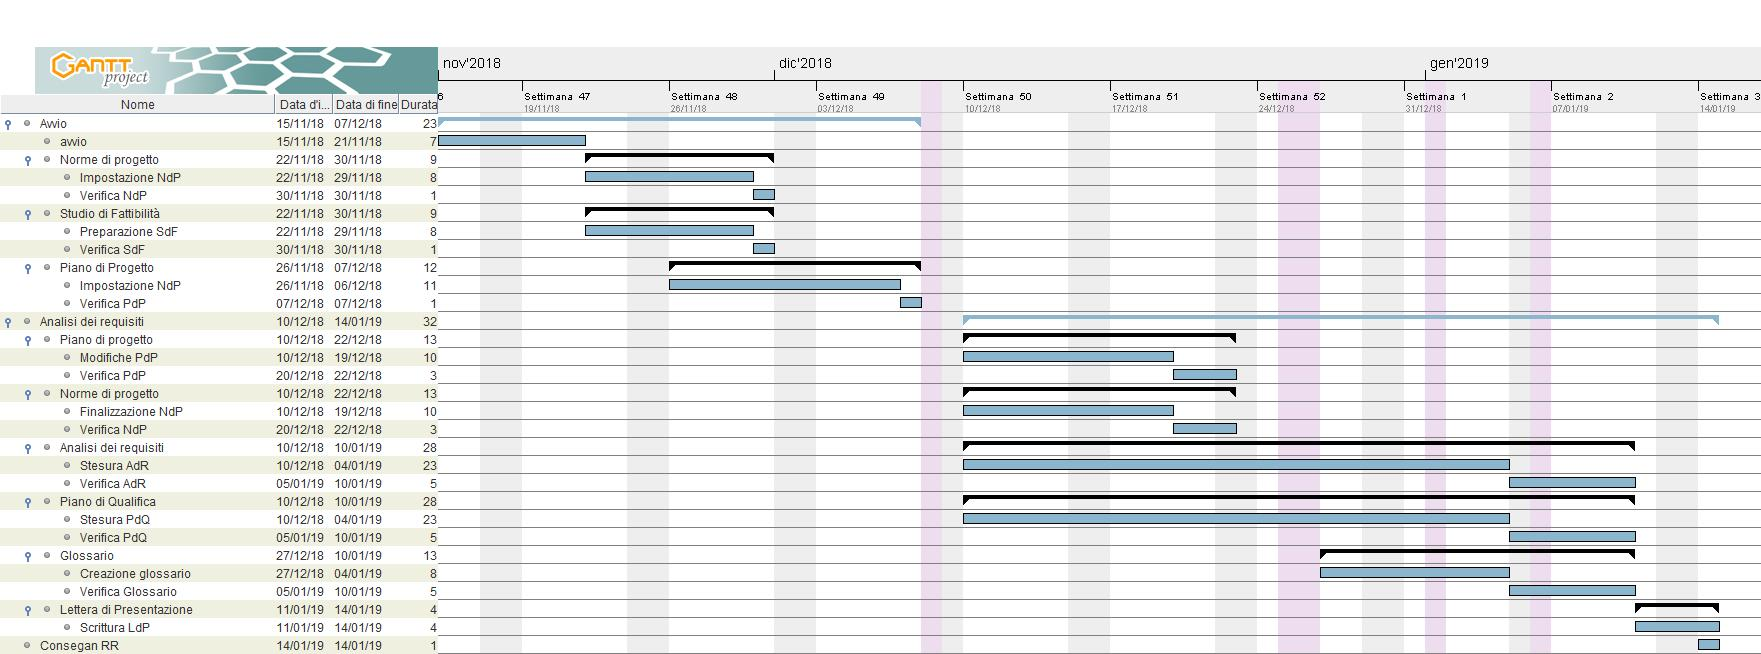
\includegraphics[width=\textwidth]{Gantt_seconda_fase.jpg}
	\caption{Diagramma di Gantt per la fase fino alla Revisione di Progettazione}
\end{figure}

\begin{figure}[h!]
	\centering
	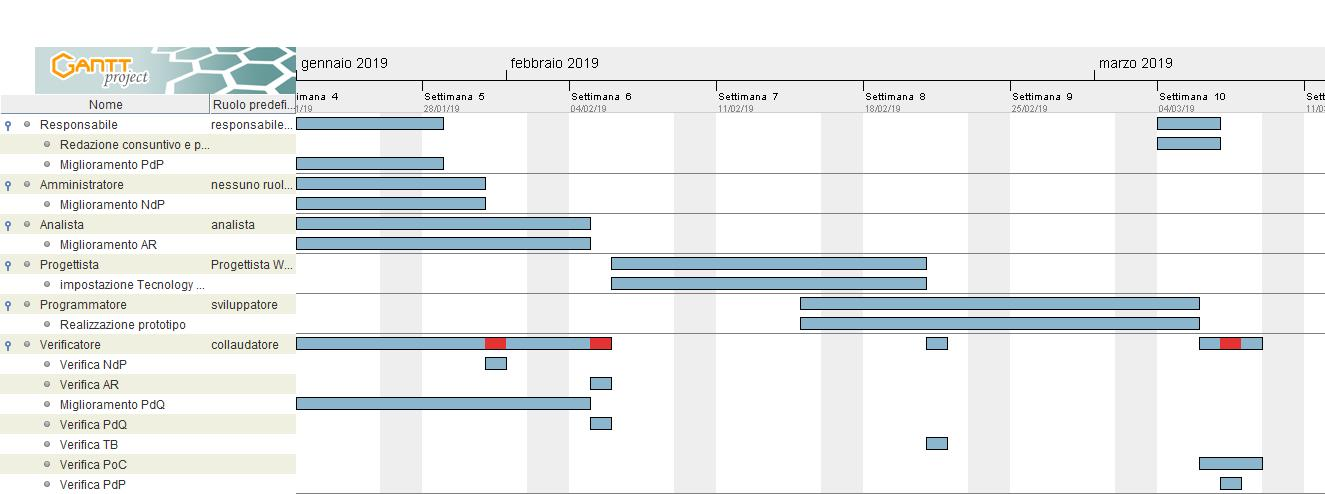
\includegraphics[width=\textwidth]{Gantt_seconda_fase_risorse.jpg}
	\caption{Diagramma di Gantt delle risorse fino alla Revisione di Progettazione}
\end{figure}

\begin{table}[h!]
	\centering
	\renewcommand{\arraystretch}{1.5}
	\begin{tabular}{|l|p{4.5cm}|p{4.5cm}|}
		\hline
		\multicolumn{3}{|c|}{\textbf{Suddivisione temporale}}\\
		\hline
		\textbf{Ruolo} & \textbf{22/01/19 - 13/02/19} & \textbf{13/2/19 - 08/03/2019} \\
		\hline
		\textbf{Responsabile} & \daL & \daG \\
		\hline
		\textbf{Amministratore} & \daG & \gia \\
		\hline
		\textbf{Analista} & \parbox{4.5cm}{\pie\\ \mic\\ \mar\\ \gia} & - \\
		\hline
		\textbf{Progettista} & \mat &  \parbox{4.5cm}{\daL \\ \mar} \\
		\hline
		\textbf{Programmatore} & - & \mic \\
		\hline
		\textbf{Verificatore} & - &  \parbox{4.5cm}{\mat \\ \pie} \\
		\hline
	\end{tabular}
	\caption{suddivisione temporale della Progettazione architetturale}
\end{table}


\subsection{Progettazione di dettaglio e codifica}
Questo periodo inizia il giorno dopo la \textit{Revisione di Progettazione}(16/03/2019) e si conclude
con la consegna dei documenti per la \textit{Revisione di Qualifica}(12/04/2019). Le attività principali sono:
\begin{itemize}
	\item{\textbf{Incremento e Verifica:} all’inizio del periodo vengono svolte attività di Incremento e Verifica su vari documenti;}
	\item{\textbf{Glossario:} questa attività comprende sia il miglioramento del Glossario che l’aggiunta di nuovi termini;}
	\item{\textbf{Codifica:} questa attività consiste nella scrittura del codice e nella sua verifica secondo quanto indicato nella \textit{Definizione di Prodotto};}
	\item{\textbf{Lettera di presentazione:} questa attività prevede la stesura della lettera
		di presentazione per la \textit{Revisione di Qualifica}.}
\end{itemize}

\begin{figure}[h!]
	\centering
	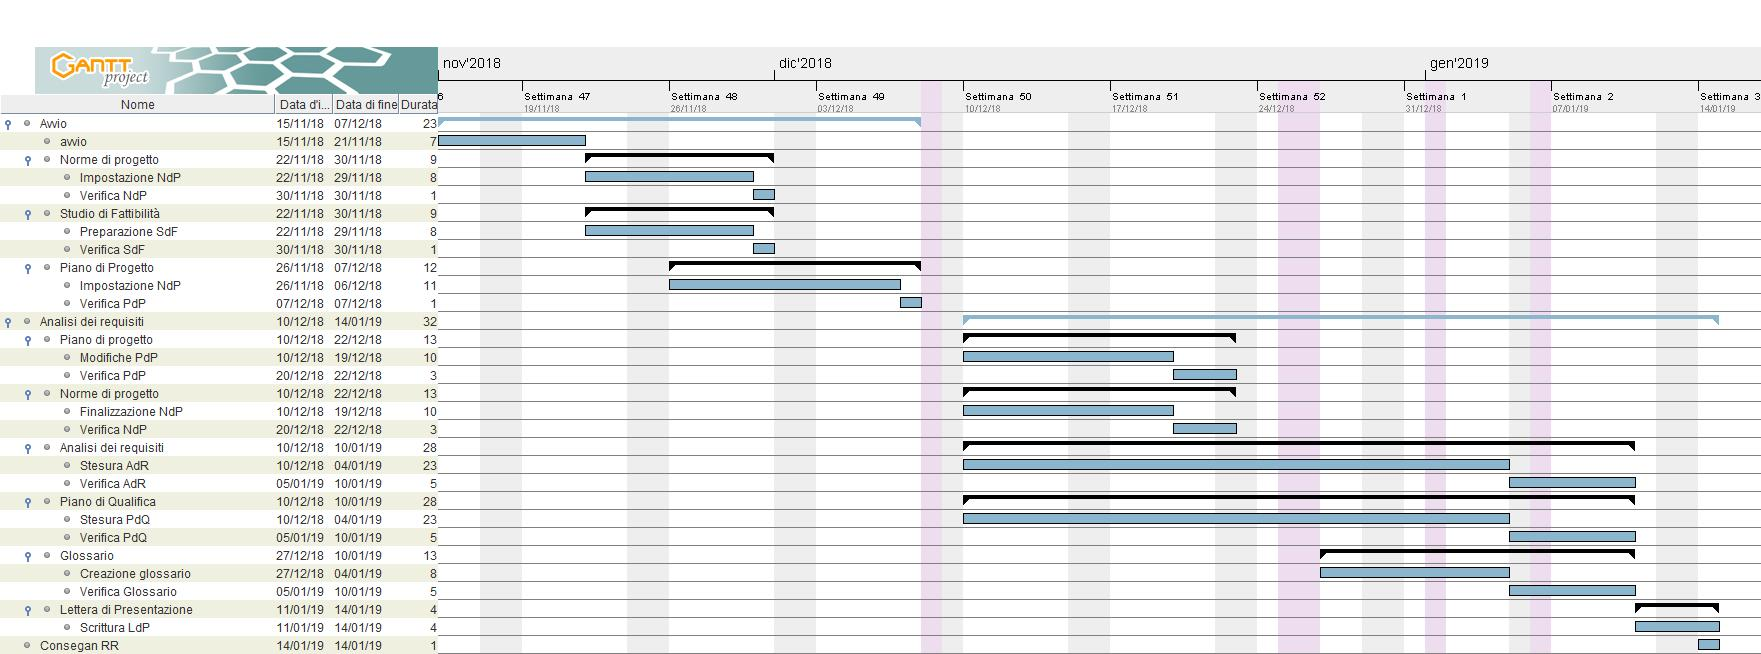
\includegraphics[width=\textwidth]{Gantt_terza_fase.jpg}
	\caption{Diagramma di Gantt per la fase fino alla Revisione di Qualifica}
\end{figure}

\begin{figure}[h!]
	\centering
	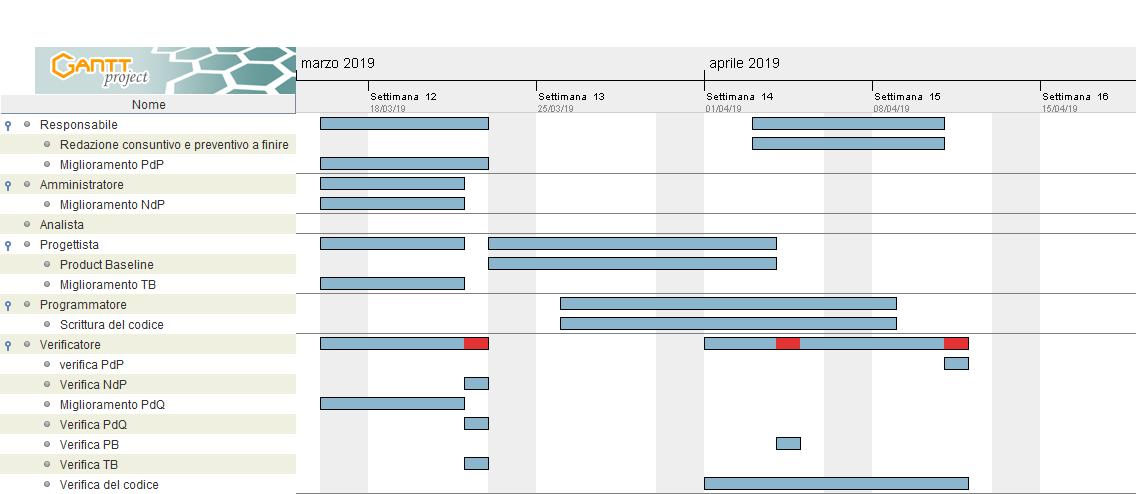
\includegraphics[width=\textwidth]{Gantt_terza_fase_risorse.jpg}
	\caption{Diagramma di Gantt delle risorse fino alla Revisione di Qualifica}
\end{figure}

\begin{tabular}{|l|l|l|}
	\hline
	\multicolumn{3}{|c|}{\textbf{Suddivisione temporale}}\\
	\hline
	\textbf{Ruolo} & \textbf{16/03/19 - 29/03/19} & \textbf{29/03/19 - 12/04/19} \\
	\hline
	\textbf{Responsabile} & \gia & \mar \\
	\hline
	\textbf{Amministratore} & \mar & \mat  \\
	\hline
	\textbf{Analista} & &  \\
	\hline
	\textbf{Progettista} & \pie \mic \daG &  \\
	\hline
	\textbf{Programmatore} & \mat \daL & \pie \daG \gia \\
	\hline
	\textbf{Verificatore} &  & \mic \daL \\
	\hline
\end{tabular}

\subsection{Validazione e collaudo}
Questo periodo inizia il giorno dopo la  \textit{Revisione di Qualifica}(20/04/2019) e si conclude con la consegna dei documenti per la  \textit{Revisione di Accettazione}(10/05/2019). 
\begin{itemize}
	\item{\textbf{Incremento e Verifica:} all’inizio del periodo vengono svolte attività di Incremento e Verifica su vari documenti;}
	\item{\textbf{Glossario:} questa attività comprende sia il miglioramento del Glossario che l’aggiunta dei nuovi termini;}
	\item{\textbf{Validazione e Collaudo:} questa attività consiste nell'attuare vari ed ulteriori test al fine di assicurare la massima qualità conforme agli obiettivi richiesti;}
	\item{\textbf{Manuale Utente:} questa attività consiste nel miglioramento e completamento del \textit{Manuale utente}, contenente indicazioni sull’utilizzo dell’applicazione.}
\end{itemize}

\begin{figure}[h!]
	\centering
	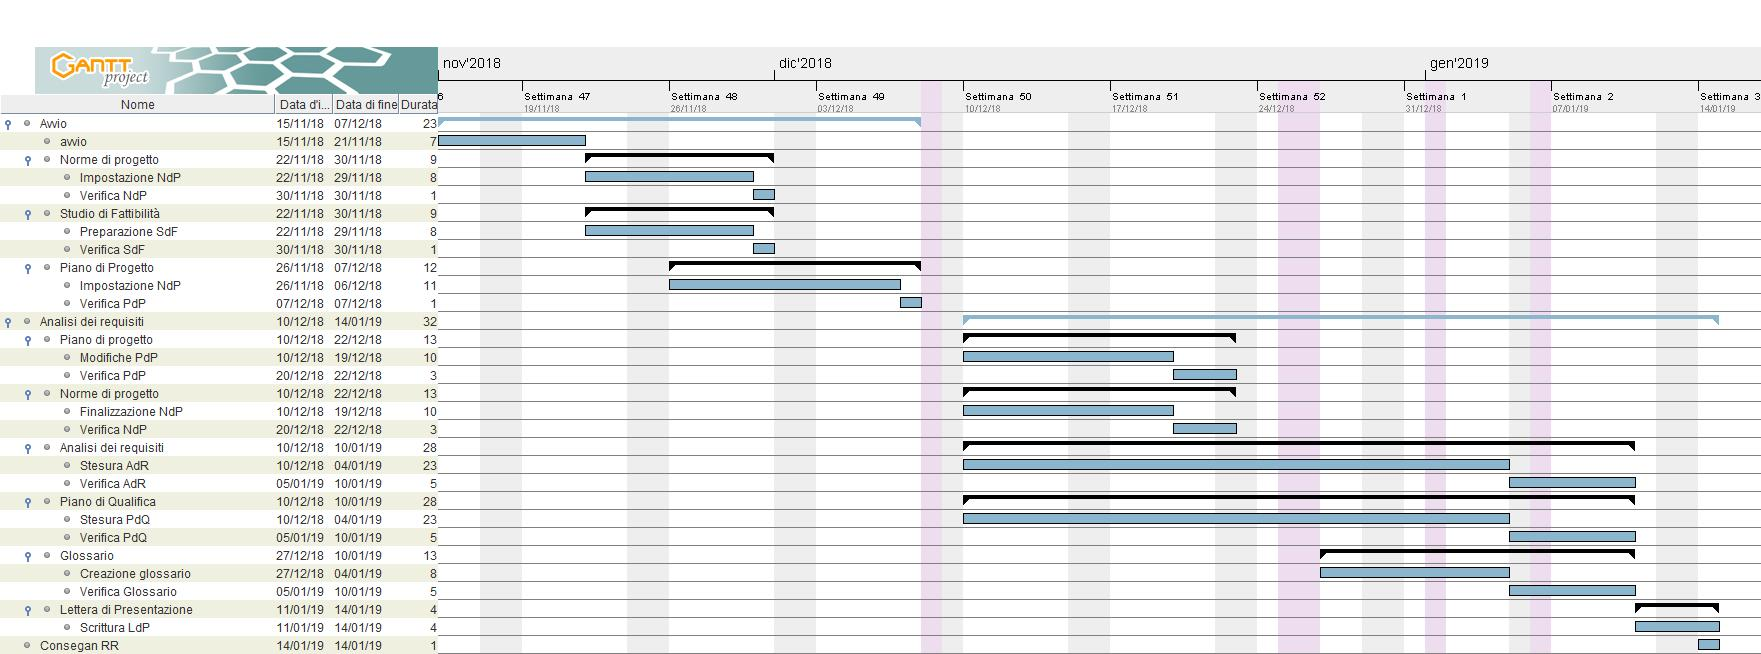
\includegraphics[width=\textwidth]{Gantt_quarta_fase.jpg}
	\caption{Diagramma di Gantt per la fase fino alla Revisione di Accettazione}
\end{figure}

\begin{figure}[h!]
	\centering
	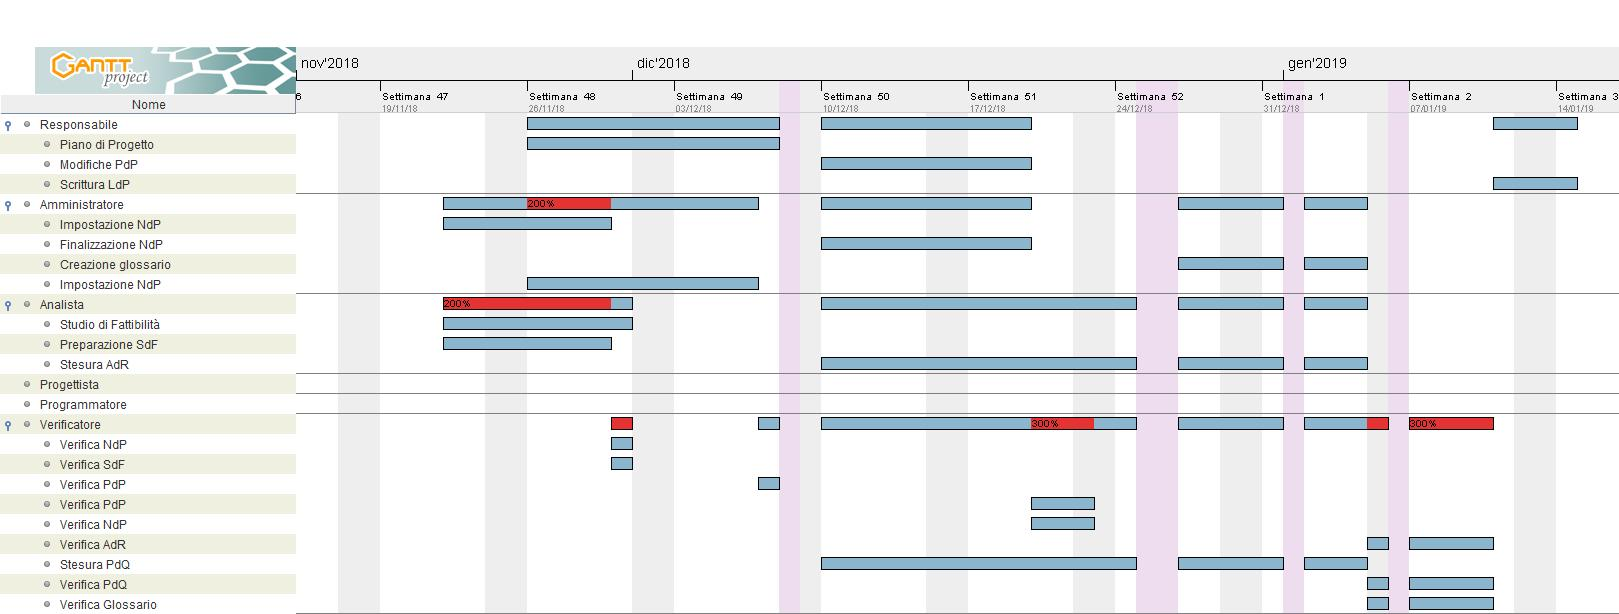
\includegraphics[width=\textwidth]{Gantt_quarta_fase_risorse.jpg}
	\caption{Diagramma di Gantt delle risorse fino alla Revisione di Accettazione}
\end{figure}

\begin{tabular}{|l|l|l|}
	\hline
	\multicolumn{3}{|c|}{\textbf{Suddivisione temporale}}\\
	\hline
	\textbf{Ruolo} & \textbf{20/04/19 - 29/04/19} & \textbf{29/04/19 - 10/05/19} \\
	\hline
	\textbf{Responsabile} & \mat  & \pie   \\
	\hline
	\textbf{Amministratore} & \pie & \mic \\
	\hline
	\textbf{Analista} & \mat \daL \daG & \pie \daG \\
	\hline
	\textbf{Progettista} & - & - \\
	\hline
	\textbf{Programmatore} & \daL \mar & - \\
	\hline
	\textbf{Verificatore} & \mic \daG \gia & \mic \mat \daL \daG \mar \gia \\
	\hline
\end{tabular}


